\documentclass{beamer}

\usepackage[utf8]{inputenc}
\usepackage{hyperref}

\usetheme{Berkeley}
\beamertemplatenavigationsymbolsempty
\setbeamertemplate{headline}{}
 
\title{FoodChain-Lab Overview}
\date{}
 
\begin{document}
\maketitle

\section{Available Nodes}
\begin{frame}
	\begin{center}
  		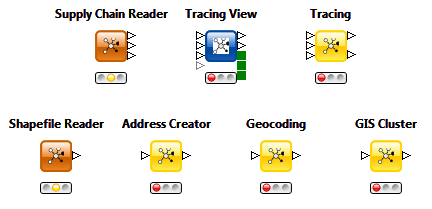
\includegraphics[height=0.4\textheight]{1.png}
	\end{center}
	\begin{itemize}
		\item Detailed descriptions all nodes are available in the \textbf{Node Description} view of KNIME.
		\item All inputs and outputs are either \textbf{data tables} (triangles) or \textbf{images} (green square). Therefore standard KNIME nodes (\textbf{Row Filter}, \textbf{Image Port Writer}, ...) can be used in FoodChain-Lab workflows.		
	\end{itemize}
\end{frame}
 
\section{Tracing}
\begin{frame}
	\begin{center}
  		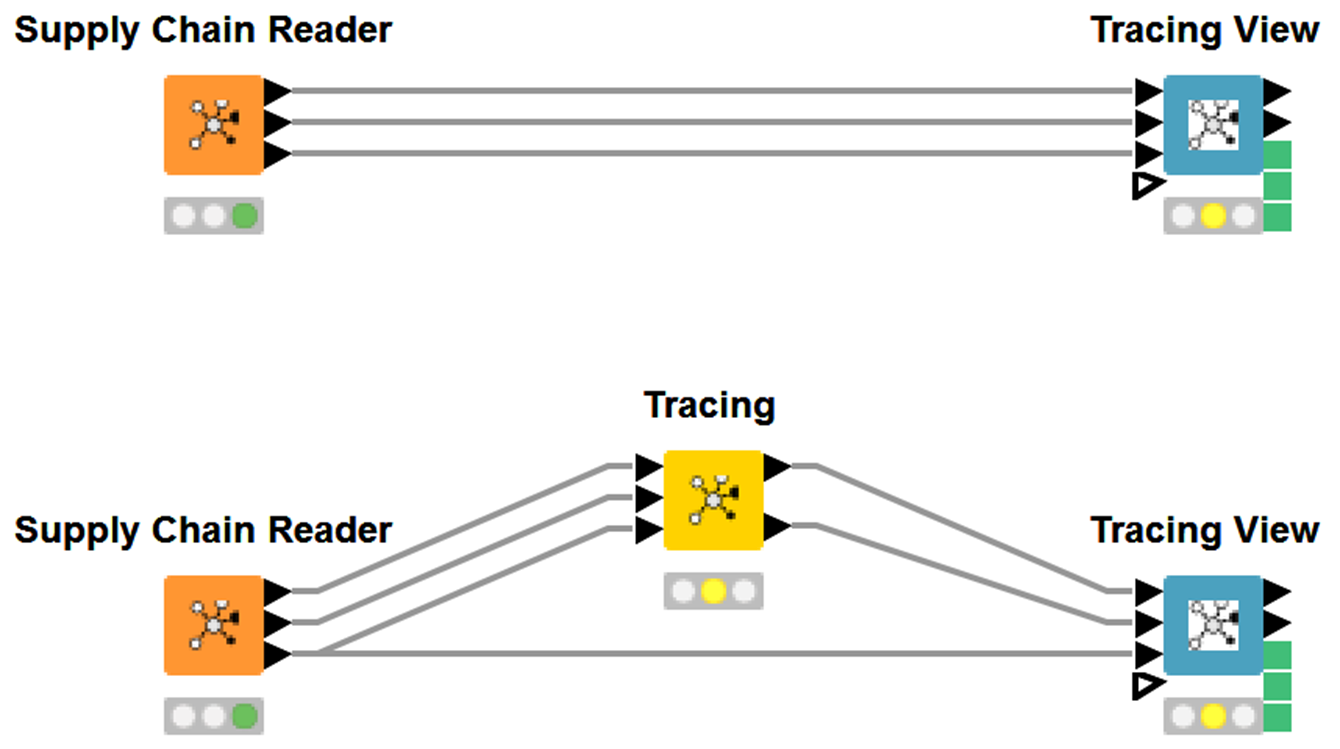
\includegraphics[height=0.4\textheight]{2.png}
	\end{center}
	\begin{itemize}
		\item Supply chain data is read from the internal database via the \textbf{Supply Chain Reader}.
		\item This data can be visualized with the \textbf{Tracing View}. The \textbf{Tracing View} also allows to perform a tracing on the data.
		\item The \textbf{Tracing} node performs tracing without visualization. Its output can be used in the \textbf{Tracing View} (e.g. to perform some tracings as a preprocessing step)
	\end{itemize}
\end{frame}

\section{Using GIS data}
\begin{frame}
	\begin{center}
  		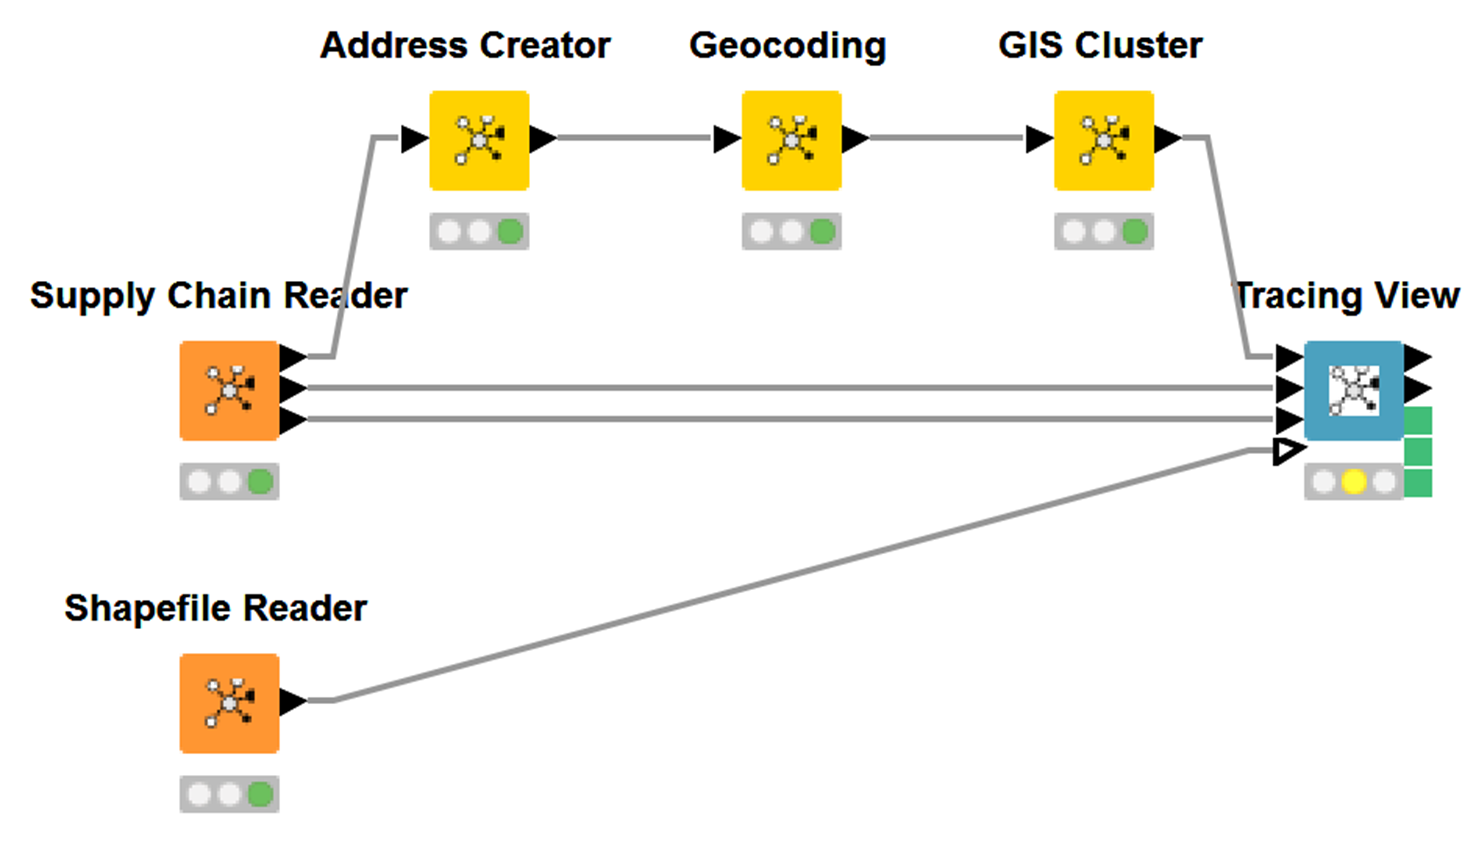
\includegraphics[height=0.6\textheight]{3.png}
	\end{center}
	\begin{itemize}
		\item The \textbf{Geocoding} node allows to acquire latitude/longitude data from addresses.
		\item This data can be geographically clustered with the \textbf{GIS Cluster} node.
		\item The \textbf{Tracing View} allows geographical visualization, if GIS data is provided from the \textbf{Shapefile Reader}.
	\end{itemize}		
\end{frame}

\end{document}